\documentclass[11pt,letterpaper]{article}

% ============================================================================
% PACKAGES
% ============================================================================
\usepackage[utf8]{inputenc}
\usepackage[T1]{fontenc}
\usepackage{helvet}
\renewcommand{\familydefault}{\sfdefault}
\usepackage[margin=0.85in, headheight=28pt]{geometry}
\usepackage{graphicx}
\usepackage{xcolor}
\usepackage{tikz}
\usepackage{tcolorbox}
\usepackage{booktabs}
\usepackage{enumitem}
\usepackage{hyperref}
\usepackage{fancyhdr}
\usepackage{titlesec}
\usepackage{multicol}
\usepackage{listings}
\usepackage{upquote}
\usepackage{amsmath,amssymb}
\usepackage{pgfplots}
\usepackage{array}
\usepackage{longtable}
\usepackage{colortbl}
\usepackage{pifont}
\usepackage{setspace}
\usepackage{parskip}
\usepackage{caption}
\usepackage{tabularx}

\pgfplotsset{compat=1.18}
\usetikzlibrary{shapes.geometric, arrows.meta, positioning, calc, decorations.pathreplacing, backgrounds, fit, shadows.blur, matrix, patterns, fadings, shadings}

% ============================================================================
% COLOR DEFINITIONS - Scientific Defense Theme (biosecurity/laboratory feel)
% ============================================================================
% Primary: Deep teal - scientific, medical, biosecurity
\definecolor{deepteal}{HTML}{0E4D4D}
\definecolor{scienceteal}{HTML}{17A2B8}
\definecolor{labcyan}{HTML}{1ABC9C}
% Accent: Barrier gold for warnings and highlights
\definecolor{barriergold}{HTML}{D4AC0D}
\definecolor{shieldamber}{HTML}{F39C12}
% Domain colors
\definecolor{biogreen}{HTML}{27AE60}
\definecolor{chemblue}{HTML}{2E86AB}
\definecolor{nukepurple}{HTML}{5B2C6F}
\definecolor{defenseblue}{HTML}{34495E}
% Neutrals
\definecolor{lightgray}{HTML}{F4F6F7}
\definecolor{medgray}{HTML}{BDC3C7}
\definecolor{softslate}{HTML}{5D6D7E}
\definecolor{textdark}{HTML}{1C2833}

% ============================================================================
% HYPERREF SETUP
% ============================================================================
\hypersetup{
  colorlinks=true,
  linkcolor=deepteal,
  urlcolor=scienceteal,
  pdftitle={AI Agents and WMD Proliferation Risk Assessment},
  pdfauthor={Emerging Technology Risk Assessment}
}

% ============================================================================
% SPACING AND TYPOGRAPHY
% ============================================================================
\setstretch{1.15}
\setlength{\parskip}{0.5em}
\setlist{nosep, leftmargin=1.5em, itemsep=0.3em}

% ============================================================================
% PAGE STYLE - Hexagonal molecular pattern (biosecurity theme)
% ============================================================================
\pagestyle{fancy}
\fancyhf{}
\fancyhead[L]{%
  \begin{tikzpicture}[baseline=-0.5ex]
    % Hexagonal pattern (molecular/biosecurity feel) - larger for visibility
    \foreach \i in {0,1,2} {
      \draw[scienceteal, opacity=0.5, line width=0.6pt]
        ({0.15+\i*0.42},0.15) -- ++(60:0.15) -- ++(0:0.15) -- ++(-60:0.15)
        -- ++(-120:0.15) -- ++(180:0.15) -- cycle;
    }
    \fill[barriergold, opacity=0.8] (0.37,0.15) circle (0.06);
  \end{tikzpicture}
  \hspace{0.4em}\textcolor{deepteal}{\textsf{\small ETRA-2025-WMD-001}}%
}
\fancyhead[R]{\textcolor{softslate}{\textsf{\thepage}}}
\fancyfoot[C]{\textcolor{softslate}{\footnotesize\textsf{Emerging Technology Risk Assessment | Biosecurity Policy Research}}}
\renewcommand{\headrulewidth}{0pt}
\renewcommand{\footrulewidth}{0pt}

\fancyheadoffset{0pt}
\setlength{\headheight}{32pt}

% ============================================================================
% SECTION FORMATTING - Scientific defense style with hexagon accents
% ============================================================================
\titleformat{\section}
  {\normalfont\LARGE\bfseries\color{deepteal}}
  {\thesection}{0.8em}{}[\vspace{-0.3em}{\color{scienceteal}\rule{\textwidth}{1.5pt}\hspace{-\textwidth}\color{barriergold}\rule{3cm}{1.5pt}}]
\titleformat{\subsection}
  {\normalfont\Large\bfseries\color{deepteal}}
  {\thesubsection}{0.6em}{}
\titleformat{\subsubsection}
  {\normalfont\large\color{softslate}\bfseries}
  {\thesubsubsection}{0.5em}{}

\titlespacing*{\section}{0pt}{3ex plus 1ex minus .2ex}{2ex plus .2ex}
\titlespacing*{\subsection}{0pt}{2.5ex plus 1ex minus .2ex}{1.5ex plus .2ex}

\setcounter{tocdepth}{2}

% ============================================================================
% TCOLORBOX ENVIRONMENTS - Scientific defense styling
% ============================================================================
\tcbuselibrary{skins,breakable,hooks}

\newtcolorbox{keybox}[1][Key Finding]{
  enhanced, breakable,
  colback=scienceteal!10, colframe=scienceteal,
  colbacktitle=scienceteal, coltitle=white,
  fonttitle=\bfseries\sffamily,
  title={\ding{72}\hspace{0.5em}#1},
  boxrule=0pt, leftrule=4pt, arc=0pt, outer arc=0pt,
  left=12pt, right=12pt, top=8pt, bottom=8pt
}

\newtcolorbox{contextbox}[1][Context]{
  enhanced, breakable,
  colback=biogreen!10, colframe=biogreen,
  colbacktitle=biogreen, coltitle=white,
  fonttitle=\bfseries\sffamily,
  title={\ding{51}\hspace{0.5em}#1},
  boxrule=0pt, leftrule=4pt, arc=0pt, outer arc=0pt,
  left=12pt, right=12pt, top=8pt, bottom=8pt
}

\newtcolorbox{notebox}[1][Note]{
  enhanced, breakable,
  colback=barriergold!12, colframe=barriergold,
  colbacktitle=barriergold, coltitle=white,
  fonttitle=\bfseries\sffamily,
  title={\ding{73}\hspace{0.5em}#1},
  boxrule=0pt, leftrule=4pt, arc=0pt, outer arc=0pt,
  left=12pt, right=12pt, top=8pt, bottom=8pt
}

\newtcolorbox{infobox}[1][Information]{
  enhanced, breakable,
  colback=chemblue!10, colframe=chemblue,
  colbacktitle=chemblue, coltitle=white,
  fonttitle=\bfseries\sffamily,
  title={\ding{73}\hspace{0.5em}#1},
  boxrule=0pt, leftrule=4pt, arc=0pt, outer arc=0pt,
  left=12pt, right=12pt, top=8pt, bottom=8pt
}

\newtcolorbox{defbox}[1][Definition]{
  enhanced, breakable,
  colback=deepteal!8, colframe=deepteal,
  colbacktitle=deepteal, coltitle=white,
  fonttitle=\bfseries\sffamily,
  title={\ding{70}\hspace{0.5em}#1},
  boxrule=0pt, leftrule=4pt, arc=0pt, outer arc=0pt,
  left=12pt, right=12pt, top=8pt, bottom=8pt
}

\newtcolorbox{quotebox}{
  enhanced, breakable,
  colback=lightgray, colframe=scienceteal!50,
  boxrule=0pt, leftrule=4pt, arc=0pt, outer arc=0pt,
  left=12pt, right=12pt, top=8pt, bottom=8pt
}

\newtcolorbox{barrierbox}[1][Barrier Analysis]{
  enhanced, breakable,
  colback=nukepurple!8, colframe=nukepurple,
  colbacktitle=nukepurple, coltitle=white,
  fonttitle=\bfseries\sffamily,
  title={\ding{74}\hspace{0.5em}#1},
  boxrule=0pt, leftrule=4pt, arc=0pt, outer arc=0pt,
  left=12pt, right=12pt, top=8pt, bottom=8pt
}

% ============================================================================
% DOCUMENT
% ============================================================================
\begin{document}

% ============================================================================
% TITLE PAGE - Concentric Defense Barriers Visualization
% ============================================================================
\begin{titlepage}

\begin{tikzpicture}[remember picture, overlay]
  % Background - deep teal gradient
  \fill[deepteal] (current page.north west) rectangle (current page.south east);

  % Hexagonal pattern background (molecular/biosecurity feel)
  \begin{scope}[shift={(current page.center)}, opacity=0.04]
    \foreach \x in {-8,-6.5,...,10} {
      \foreach \y in {-12,-10.5,...,12} {
        \draw[white, line width=0.3pt]
          (\x,\y) -- ++(60:0.5) -- ++(0:0.5) -- ++(-60:0.5)
          -- ++(-120:0.5) -- ++(180:0.5) -- cycle;
      }
    }
  \end{scope}

  % Main visualization - Concentric Defense Barriers
  \begin{scope}[shift={([xshift=-0.3cm, yshift=1.2cm]current page.center)}]
    % Outer barrier ring (weakest - eroding) with label
    \draw[labcyan, opacity=0.15, line width=8pt] (0,0) circle (5.5cm);
    \draw[labcyan, opacity=0.25, line width=2pt, dashed] (0,0) circle (5.5cm);
    \node[white, opacity=0.6, font=\fontsize{6}{6}\selectfont\sffamily, rotate=-20] at (50:5.9cm) {INFORMATION BARRIER};

    % Middle barrier ring (moderate) with label
    \draw[scienceteal, opacity=0.2, line width=10pt] (0,0) circle (4cm);
    \draw[scienceteal, opacity=0.4, line width=2pt] (0,0) circle (4cm);
    \node[white, opacity=0.6, font=\fontsize{6}{6}\selectfont\sffamily, rotate=15] at (130:4.4cm) {PHYSICAL BARRIER};

    % Inner barrier ring (strong) with label
    \draw[barriergold, opacity=0.25, line width=12pt] (0,0) circle (2.5cm);
    \draw[barriergold, opacity=0.6, line width=2pt] (0,0) circle (2.5cm);
    \node[white, opacity=0.7, font=\fontsize{6}{6}\selectfont\sffamily, rotate=-30] at (-40:2.9cm) {TACIT KNOWLEDGE};

    % Core - protected zone
    \fill[white, opacity=0.1] (0,0) circle (1.3cm);
    \fill[barriergold] (0,0) circle (0.8cm);
    \node[deepteal, font=\fontsize{7}{7}\selectfont\bfseries] at (0,0.12) {DEFENSE};
    \node[deepteal, font=\fontsize{7}{7}\selectfont\bfseries] at (0,-0.18) {IN DEPTH};

    % Domain nodes - evenly distributed on outer ring
    \foreach \angle/\col/\label in {
      0/biogreen/BIO,
      45/labcyan/SCREEN,
      90/scienceteal/DETECT,
      135/chemblue/CHEM,
      180/nukepurple/NUKE,
      225/shieldamber/GOVERN,
      270/barriergold/ATTRIB,
      315/biogreen/INTL
    } {
      \fill[\col, opacity=0.9] (\angle:5.5cm) circle (0.4cm);
      \node[white, font=\fontsize{5}{5}\selectfont\bfseries] at (\angle:5.5cm) {\label};
    }

    % Breach indicators (showing where barriers are weakening)
    \foreach \angle in {22.5, 67.5, 112.5, 157.5, 202.5, 247.5, 292.5, 337.5} {
      \draw[white, opacity=0.25, line width=0.8pt, ->] (\angle:6.3cm) -- (\angle:5.9cm);
    }
  \end{scope}

  % Document header bar (keeping consistent format)
  \fill[barriergold] ([yshift=-1.5cm]current page.north west) rectangle ([yshift=-2.2cm]current page.north east);
  \node[deepteal, font=\small\bfseries\sffamily] at ([yshift=-1.85cm]current page.north) {PROJECTION REPORT \textbar{} ETRA-2025-WMD-001 \textbar{} DECEMBER 2025};

  % Title block
  \node[anchor=south west, text width=14cm] at ([xshift=1.5cm, yshift=3cm]current page.south west) {
    {\fontsize{11}{13}\selectfont\color{barriergold}\sffamily EMERGING TECHNOLOGY RISK ASSESSMENT}\\[0.8cm]
    {\fontsize{36}{42}\selectfont\bfseries\color{white}AI Agents and}\\[0.2cm]
    {\fontsize{36}{42}\selectfont\bfseries\color{white}WMD Proliferation}\\[0.2cm]
    {\fontsize{36}{42}\selectfont\bfseries\color{white}Risk}\\[0.6cm]
    {\large\color{medgray}\sffamily A Policy Research Document on Defensive Preparedness}
  };

  % Metadata block
  \node[anchor=south east, text width=5cm, align=right] at ([xshift=-1.5cm, yshift=3cm]current page.south east) {
    \color{softslate}\small\sffamily
    \textbf{Document Type:} Policy Research\\[0.2em]
    \textbf{Time Horizon:} 2025--2030\\[0.2em]
    \textbf{License:} MIT / Unlicense\\[0.2em]
    \textbf{Version:} 2.0
  };

  % Accent line
  \draw[barriergold, line width=2pt] ([xshift=1.5cm, yshift=3cm]current page.south west) -- ([xshift=1.5cm, yshift=10.5cm]current page.south west);

\end{tikzpicture}
\end{titlepage}

% ============================================================================
% ABOUT THIS DOCUMENT
% ============================================================================
\thispagestyle{empty}
\vspace*{0.5cm}

\noindent\begin{tikzpicture}
  \fill[deepteal] (0,0) rectangle (\textwidth, 0.2);
  % Hexagonal accent pattern - larger for visibility
  \foreach \x in {0.4,1.0,...,16.5} {
    \draw[barriergold, opacity=0.7, line width=0.5pt]
      (\x, 0.1) -- ++(60:0.08) -- ++(0:0.08) -- ++(-60:0.08)
      -- ++(-120:0.08) -- ++(180:0.08) -- cycle;
  }
\end{tikzpicture}

\vspace{0.5cm}
\begin{center}
{\color{deepteal}\Large\bfseries About This Document}
\end{center}
\vspace{0.3cm}

\begin{tcolorbox}[enhanced, colback=lightgray, colframe=scienceteal!60, boxrule=1pt, arc=3pt,
  left=10pt, right=10pt, top=10pt, bottom=10pt]
This is a \textbf{public policy research document} analyzing how AI capabilities may affect WMD proliferation risks. It is released under permissive open-source licenses (MIT/Unlicense) to support broad discussion of these governance challenges.
\end{tcolorbox}

\vspace{0.5cm}

\begin{minipage}[t]{0.48\textwidth}
\textbf{Intended Audiences:}
\begin{itemize}[nosep]
  \item Policy researchers and analysts
  \item AI safety and security researchers
  \item Academic communities studying technology governance
  \item Journalists covering AI risks
  \item General public interested in emerging technology policy
\end{itemize}
\end{minipage}
\hfill
\begin{minipage}[t]{0.48\textwidth}
\textbf{How to Use This Document:}
\begin{itemize}[nosep]
  \item The analysis is framed for \textit{defensive} purposes
  \item Technical details that could enable harm are intentionally omitted
  \item Probability estimates are discussion aids, not predictions
  \item When excerpting, please preserve context
\end{itemize}
\end{minipage}

\vspace{0.8cm}

\begin{contextbox}[What This Document Is NOT Claiming]
To prevent misreading, we explicitly clarify:
\begin{itemize}
  \item \textbf{NOT claiming an imminent WMD wave.} Actual WMD attacks by non-state actors remain extremely rare. Our assessment is that \textit{attempt frequency} may increase while \textit{success rate} remains low.
  \item \textbf{NOT claiming novices can build WMD.} AI does not transform a curious novice (T0) into a capable threat actor. The primary effect is upgrading T1--T3 actors who already have partial capability.
  \item \textbf{NOT claiming AI is the dominant proliferation driver.} Geopolitics, state programs, and traditional pathways remain more significant than AI-enabled non-state threats in most scenarios.
  \item \textbf{NOT claiming restriction-only solutions work.} Effective strategy requires balanced investment in detection, attribution, response, and resilience.
  \item \textbf{NOT claiming high confidence in probability estimates.} Scenario probabilities are subjective priors for decision support, not empirical predictions.
\end{itemize}
\end{contextbox}

\vspace{0.5cm}

\begin{infobox}[Epistemic Status Markers]
Throughout this document, key claims are tagged with epistemic status:
\begin{center}
\small
\begin{tabular}{p{1.5cm}p{4cm}p{6cm}}
\toprule
\textbf{Marker} & \textbf{Meaning} & \textbf{Evidence Standard} \\
\midrule
\textbf{[O]} & Open-source documented & Published research, official statements, public data \\
\textbf{[E]} & Expert judgment & Consistent with theory and limited evidence; gaps acknowledged \\
\textbf{[S]} & Speculative projection & Extrapolation from trends; significant uncertainty \\
\bottomrule
\end{tabular}
\end{center}
\end{infobox}

\newpage

% ============================================================================
% EXECUTIVE SUMMARY
% ============================================================================
\section*{Executive Summary}
\addcontentsline{toc}{section}{Executive Summary}

This projection examines how autonomous AI agents may alter the proliferation landscape for weapons of mass destruction (WMD). We analyze current technological capabilities as of late 2025, project scenarios through 2030, and examine the interplay between AI capabilities, existing physical barriers, and potential defensive adaptations.

\begin{keybox}[Key Findings]
\begin{enumerate}
  \item \textbf{[E]} Agentic AI workflows are unlikely to enable a novice to construct a functional WMD, but they will meaningfully lower barriers for actors who already have partial capability (T1--T3)
  \item \textbf{[E]} Biological weapons represent the highest-risk category due to eroding physical barriers and AI's strength in knowledge synthesis
  \item \textbf{[E]} The ``tacit knowledge gap'' remains significant, but AI-guided systems and cloud labs are beginning to erode it
  \item \textbf{[O]} Nuclear weapons face the strongest physical barriers; AI primarily assists state-level programs
  \item \textbf{[E]} The most likely scenario is high-frequency attempts with limited success---resource strain and public concern, not mass casualties
\end{enumerate}
\end{keybox}

\subsection*{Why Now? Capability Shift 2023--2025}

\begin{center}
\small
\begin{tabular}{p{3cm}p{4cm}p{4cm}p{2.5cm}}
\toprule
\textbf{Capability} & \textbf{2023 State} & \textbf{2025 State} & \textbf{Impact} \\
\midrule
Agentic autonomy & Chatbots provided info & Agents execute multi-step tasks \textbf{[O]} & Knowledge $\to$ execution \\
Vision-language & Text-only instruction & Real-time visual interpretation \textbf{[O]} & Bridges tacit knowledge \\
Computer Use & Manual web interaction & Agents browse, fill forms \textbf{[O]} & Procurement automation \\
Biological design & AlphaFold 2 (structure) & AlphaFold 3, ESM3 (generative) \textbf{[O]} & Optimization capability \\
Open-weight models & Limited high-capability & Llama 3, Mistral, fine-tuning \textbf{[O]} & Guardrail bypass potential \\
\bottomrule
\end{tabular}
\end{center}

\subsection*{Base-Rate Context: Anchoring Expectations}

\begin{quotebox}
\textbf{Actual WMD attacks by non-state actors remain extremely rare.} The 1995 Tokyo subway attack and 2001 anthrax letters represent essentially the entire modern history of non-state WMD use. The overwhelming majority of WMD-related arrests involve early-stage planning with minimal actual capability.

The dominant near-term concern is \textit{increased frequency of attempts} with varying competence, not catastrophic mass-casualty events. Readers should interpret this analysis through that lens.
\end{quotebox}

\newpage
\tableofcontents
\newpage

% ============================================================================
% ONE-PAGE EXECUTIVE SUMMARY
% ============================================================================
\section*{Quick Reference: One-Page Summary}
\addcontentsline{toc}{section}{Quick Reference: One-Page Summary}

\subsection*{Core Claims}

\begin{enumerate}
  \item \textbf{Biological weapons are the highest-risk category} for AI-enabled proliferation due to eroding physical barriers and high AI contribution to knowledge synthesis
  \item \textbf{AI primarily upgrades T1--T3 actors} (skilled individuals to organized groups); it does not transform novices into capable threat actors
  \item \textbf{The most likely near-term scenario is high-frequency attempts with limited success}---resource strain and public concern, not mass casualties
  \item \textbf{Cyber-physical attacks on existing infrastructure} (labs, chemical plants) may be higher-leverage than synthesis assistance
  \item \textbf{Governance windows are closing}---once capabilities proliferate, restrictions become harder to implement
\end{enumerate}

\subsection*{Top 5 Recommended Actions}

\begin{enumerate}
  \item \textbf{Mandate universal DNA synthesis screening} with international harmonization
  \item \textbf{Invest in attribution and response capabilities}---cannot rely on deterrence alone
  \item \textbf{Establish cloud laboratory oversight frameworks} before the attack surface expands further
  \item \textbf{Require WMD-relevant capability evaluations} before frontier AI deployment
  \item \textbf{Fund defensive biodetection} as a high-value cross-threat investment
\end{enumerate}

\subsection*{Top 5 Indicators to Monitor}

\begin{enumerate}
  \item DNA synthesis screening intercept rates and patterns
  \item AI model performance on biology/chemistry benchmarks
  \item Cloud laboratory service expansion and security posture
  \item Dark web discussion of AI + WMD capabilities
  \item Progress (or lack thereof) on international governance coordination
\end{enumerate}

\subsection*{What Would Change This Assessment}

\begin{minipage}[t]{0.48\textwidth}
\textbf{Would Increase Concern:}
\begin{itemize}[nosep]
  \item Confirmed AI-assisted WMD attempt
  \item Release of unrestricted biology-capable research agent
  \item Major cloud lab security breach
\end{itemize}
\end{minipage}
\hfill
\begin{minipage}[t]{0.48\textwidth}
\textbf{Would Decrease Concern:}
\begin{itemize}[nosep]
  \item Effective international AI safety framework
  \item Robust attribution breakthrough
  \item AI guardrails prove more durable than expected
\end{itemize}
\end{minipage}

\newpage

% ============================================================================
% PART I - FOUNDATIONS
% ============================================================================
\clearpage
\thispagestyle{empty}
\vspace*{-0.85in}
\noindent\hspace*{-0.85in}\begin{tikzpicture}
  \fill[deepteal] (0,0) rectangle (\paperwidth, -10cm);

  \node[barriergold, font=\fontsize{10}{10}\selectfont\sffamily] at (0.5\paperwidth, -1.2cm) {PART I};
  \node[white, font=\fontsize{48}{48}\selectfont\bfseries] at (0.5\paperwidth, -2.8cm) {Foundations};
  \node[white, opacity=0.7, font=\normalsize\sffamily] at (0.5\paperwidth, -4.2cm) {Theory, Capabilities, and Historical Context};

  % Concentric barrier rings visualization (unique to WMD doc)
  \begin{scope}[shift={(4cm, -7.5cm)}]
    % Three concentric rings representing defense layers
    \draw[labcyan, opacity=0.25, line width=6pt] (0,0) circle (2.2cm);
    \draw[labcyan, opacity=0.4, line width=1.5pt, dashed] (0,0) circle (2.2cm);
    \draw[scienceteal, opacity=0.35, line width=5pt] (0,0) circle (1.5cm);
    \draw[scienceteal, opacity=0.55, line width=1.5pt] (0,0) circle (1.5cm);
    \draw[barriergold, opacity=0.5, line width=4pt] (0,0) circle (0.8cm);
    \draw[barriergold, opacity=0.8, line width=1.5pt] (0,0) circle (0.8cm);
    \fill[barriergold, opacity=0.95] (0,0) circle (0.35cm);
    % Sector labels - positioned along rings with better readability
    \node[white, opacity=0.8, font=\fontsize{6}{6}\selectfont\sffamily, anchor=west] at (-3.5, 2.2) {INFO};
    \node[white, opacity=0.8, font=\fontsize{6}{6}\selectfont\sffamily, anchor=west] at (-3.5, 1.5) {PHYS};
    \node[white, opacity=0.8, font=\fontsize{6}{6}\selectfont\sffamily, anchor=west] at (-3.5, 0.8) {TACIT};
    % Connector lines to rings
    \draw[white, opacity=0.3, line width=0.5pt] (-3.0, 2.2) -- (-2.2, 2.2);
    \draw[white, opacity=0.3, line width=0.5pt] (-3.0, 1.5) -- (-1.5, 1.5);
    \draw[white, opacity=0.3, line width=0.5pt] (-3.0, 0.8) -- (-0.8, 0.8);
  \end{scope}

  % Legend
  \node[white, opacity=0.5, font=\fontsize{7}{7}\selectfont, anchor=west] at (10cm, -5.7cm) {DEFENSE IN DEPTH MODEL};
  \node[anchor=west] at (10cm, -6.4cm) {
    \begin{tikzpicture}
      \fill[biogreen, opacity=0.7] (0,0) circle (0.1);
      \node[white, opacity=0.7, font=\fontsize{7}{7}\selectfont, anchor=west] at (0.25, 0) {Biological - Barriers Eroding};
    \end{tikzpicture}
  };
  \node[anchor=west] at (10cm, -7.0cm) {
    \begin{tikzpicture}
      \fill[nukepurple, opacity=0.7] (0,0) circle (0.1);
      \node[white, opacity=0.7, font=\fontsize{7}{7}\selectfont, anchor=west] at (0.25, 0) {Nuclear - Barriers Strong};
    \end{tikzpicture}
  };

  \fill[barriergold] (2cm, -9.2cm) rectangle (\paperwidth-2cm, -9.3cm);
\end{tikzpicture}

\vspace{0.8cm}

\section{Introduction and Methodology}

\subsection{Purpose}

The development of weapons of mass destruction has historically required either state-level resources or exceptional individual expertise. The Manhattan Project employed over 125,000 people. Aum Shinrikyo, despite millions of dollars and multiple PhD scientists, failed to effectively weaponize biological agents.

We are now entering an era where autonomous AI agents capable of complex multi-step planning become widely accessible. This projection examines whether and how AI agents might erode these historical barriers.

\textbf{Critical framing}: This analysis does not assume WMD attacks will increase. The goal is to understand how AI capabilities change the \textit{nature} of proliferation risks, identify which categories face the greatest barrier reduction, and recommend defensive preparations.

\subsection{Methodology}

This analysis draws on:
\begin{itemize}
  \item \textbf{Current capability assessment} of AI systems and synthetic biology tools as deployed in late 2025
  \item \textbf{Historical case analysis} of WMD development programs (state and non-state)
  \item \textbf{Dual-Use Research of Concern (DURC)} literature and policy debates
  \item \textbf{Expert consultation} across biosecurity, nuclear security, and AI safety domains
  \item \textbf{Red team exercises} examining potential applications (conducted under controlled conditions)
\end{itemize}

We deliberately avoid: specific technical implementation details, named pathogen sequences or synthesis routes, and information not already publicly available in academic literature.

\subsection{What We've Observed in 2025}

Evidence regarding AI-assisted biosecurity threats, categorized by epistemic status:

\textbf{Demonstrated in open evaluations:}
\begin{itemize}[nosep]
  \item AI models can provide general information about pathogen biology from open literature
  \item Frontier AI models refuse most explicit requests for weapons guidance but inconsistencies exist
  \item AI systems show measurable ``uplift'' in non-expert comprehension of complex biological concepts
\end{itemize}

\textbf{Supported by limited disclosures:}
\begin{itemize}[nosep]
  \item DNA synthesis screening has intercepted concerning orders (industry statements, limited specifics)
  \item Security services have begun integrating AI into threat monitoring
\end{itemize}

\textbf{Speculative / emerging:}
\begin{itemize}[nosep]
  \item AI-enabled gain-of-function design assistance (theoretical capability, no documented attempts)
  \item Cloud laboratory exploitation for harmful protocols (no known incidents)
\end{itemize}

\textbf{Absence of evidence (notable):}
\begin{itemize}[nosep]
  \item No documented cases of AI-enabled biological weapon development
  \item No confirmed AI-assisted WMD attacks or advanced attempts
\end{itemize}

\subsection{Definitions}

\begin{defbox}[Core Definitions]
\textbf{Chatbot vs. Autonomous Research Agent} (critical 2025 distinction):

\vspace{0.5em}
\begin{center}
\small
\begin{tabular}{p{3cm}p{5cm}p{4cm}}
\toprule
\textbf{Type} & \textbf{Capability} & \textbf{Risk Profile} \\
\midrule
Chatbot (2022--23) & Provides information; no tool use; no persistence & Knowledge aggregation only \\
Autonomous Agent (2024--25) & Multi-step tasks; tools; self-correction; context persistence & Shifts knowledge to execution \\
\bottomrule
\end{tabular}
\end{center}

\vspace{0.5em}
\textbf{Biological Design Tools (BDTs)}: Specialized AI models for biological research (AlphaFold 3, ESM3, RFdiffusion). Often fewer guardrails than consumer chatbots.

\vspace{0.5em}
\textbf{Computer Use Capabilities}: AI agents interacting with GUIs, browsing, filling forms (Claude computer use, OpenAI Operator). Enables autonomous procurement.

\vspace{0.5em}
\textbf{Uplift}: The degree to which AI assistance improves a non-expert's ability to accomplish a dangerous task.
\end{defbox}

\subsection{Threat Actor Taxonomy}

To avoid the misleading implication that ``AI democratizes WMD to everyone,'' this report uses a tiered actor model:

\begin{center}
\small
\begin{tabular}{p{1cm}p{3.5cm}p{3.5cm}p{4cm}}
\toprule
\textbf{Tier} & \textbf{Description} & \textbf{Pre-AI Capability} & \textbf{Examples} \\
\midrule
T0 & Curious novice & No practical capability & Online researchers \\
T1 & Skilled individual with access & Limited by knowledge gaps & Disgruntled lab worker \\
T2 & Small funded group & Constrained by coordination & Extremist cell \\
T3 & Organized non-state & Historically capable (Aum) & Terrorist organizations \\
T4 & State or state-backed & Full WMD capability & Nation-state programs \\
\bottomrule
\end{tabular}
\end{center}

\textbf{Key insight}: AI primarily benefits T1--T3 actors by reducing knowledge aggregation barriers---it does not transform T0 into T3.

\subsection{Vision-Language Models and Tacit Knowledge Erosion}

The traditional ``tacit knowledge'' barrier assumed that laboratory skills require hands-on training. Vision-Language Models (VLMs) that can ``see'' through cameras are beginning to erode this barrier.

\begin{center}
\small
\begin{tabular}{p{3.5cm}p{4cm}p{4.5cm}}
\toprule
\textbf{VLM Generation} & \textbf{Capability} & \textbf{Tacit Knowledge Impact} \\
\midrule
Text-only LLMs (2022--23) & Written instruction only & Cannot interpret physical observations \\
Basic VLMs (2024) & Static image interpretation & Can identify equipment, reagents \\
Advanced VLMs (2025) & Real-time video analysis & Can provide feedback on ongoing procedures \\
Projected (2026+) & Integrated lab automation & Direct control of robotic systems \\
\bottomrule
\end{tabular}
\end{center}

\textbf{Visual Troubleshooting Scenario} (for defender awareness): Smart glasses can stream video to cloud VLMs \textbf{[O]}. An actor could receive real-time audio feedback while performing procedures. VLM interprets visual state (``color too dark,'' ``precipitate forming'') and suggests adjustments \textbf{[E]}. This partially substitutes for the mentor-mentee relationship that traditionally transmitted tacit knowledge.

\textbf{Current limitation} \textbf{[E]}: VLMs still make errors on domain-specific interpretation; a failed procedure may be unrecoverable. But the gap is narrowing with each model generation.

\subsection{Governance Challenge: Open-Weight Models}

Most AI safety measures exist at the API level for closed commercial models. Open-weight models present a distinct governance challenge:

\begin{center}
\small
\begin{tabular}{p{3cm}p{2cm}p{2cm}p{2cm}p{3cm}}
\toprule
\textbf{Model Type} & \textbf{Guardrails} & \textbf{Monitoring} & \textbf{Fine-tuning} & \textbf{Governance Lever} \\
\midrule
Closed API (GPT, Claude) & Strong & Yes & No & Provider responsibility \\
Open-weight (Llama, Mistral) & Varies & No (local) & Yes & Release decisions only \\
Fine-tuned variants & Often removed & No & Already done & Difficult to control \\
Specialized biology models & May be absent & No & Domain-specific & Research community norms \\
\bottomrule
\end{tabular}
\end{center}

\textbf{Policy implications}: (1) Pre-release capability evaluation, (2) Compute governance as monitoring opportunity, (3) Community norms on responsible release, (4) Accept that some proliferation is unavoidable---invest in detection accordingly.

\section{Theoretical Frameworks}

\subsection{Unified Risk Model}

\begin{center}
\fbox{\parbox{0.85\textwidth}{
\centering
\textbf{Risk = Capability $\times$ Access $\times$ Intent $\times$ Execution $\times$ (1 $-$ Interdiction) $\times$ Impact}
}}
\end{center}

\begin{center}
\small
\begin{tabular}{p{3cm}p{3.5cm}p{2.5cm}p{2.5cm}}
\toprule
\textbf{Factor} & \textbf{AI Contribution} & \textbf{Bio (2025--30)} & \textbf{Nuke (2025--30)} \\
\midrule
Capability (can attempt) & HIGH (knowledge synthesis) & Rising & Stable \\
Access (materials/tools) & MEDIUM (cloud labs) & Rising & Stable (fissile) \\
Intent (motivation) & NONE (AI doesn't create) & Stable & Stable \\
Execution (attempt success) & MEDIUM (guidance) & Rising slowly & Stable \\
Interdiction (detection) & MIXED (both sides) & Declining pressure & Stable (strong) \\
\bottomrule
\end{tabular}
\end{center}

\textbf{Key insight}: AI primarily affects Capability and Access (cognitive barriers). Physical barriers, Intent, and Impact Scale are largely AI-independent.

\subsection{The Tacit Knowledge Gap}

\textbf{Michael Polanyi's concept of tacit knowledge}---skills that cannot be fully articulated and must be learned through practice---is central to understanding WMD barriers. Much of weapons development relies on sensory cues, equipment calibration, and ``laboratory intuition'' accumulated over years.

AI agents can transmit explicit knowledge but traditionally cannot transfer tacit knowledge. However, two developments challenge this:
\begin{enumerate}
  \item \textbf{AI-guided instruction}: Real-time guidance that interprets user observations
  \item \textbf{Cloud laboratories}: Robotic systems that embody tacit knowledge in automated protocols
\end{enumerate}

\subsection{Offense-Defense Balance}

\begin{center}
\small
\begin{tabular}{p{4cm}p{4cm}p{4cm}}
\toprule
\textbf{Factor} & \textbf{Favors Offense} & \textbf{Favors Defense} \\
\midrule
Knowledge accessibility & AI aggregates dispersed information & AI can detect dangerous queries \\
Physical materials & Some barriers eroding (DNA synthesis) & Nuclear/chemical materials controlled \\
Attribution & AI complicates attribution & AI forensics improving \\
Detection & Novel agents may evade detection & AI-enhanced surveillance possible \\
\bottomrule
\end{tabular}
\end{center}

The balance varies significantly across WMD categories, which is why biological, chemical, and nuclear require separate analysis.

\subsection{2024--2025 Policy Developments}

\begin{center}
\small
\begin{tabular}{p{4cm}p{2cm}p{6cm}}
\toprule
\textbf{Reference} & \textbf{Date} & \textbf{Relevance} \\
\midrule
Bletchley Declaration & Nov 2023 & First international consensus on AI risks including CBRN \textbf{[O]} \\
Seoul AI Safety Summit & May 2024 & Extended Bletchley with specific bio-risk language \textbf{[O]} \\
US Executive Order 14110 & Oct 2023 & Mandates evaluation of AI role in CBRN threats \textbf{[O]} \\
RAND ``Operational Risks'' & 2024 & Definitive uplift study finding limited current risk \textbf{[O]} \\
Anthropic RSP Framework & 2023--24 & Responsible Scaling Policy with CBRN thresholds \textbf{[O]} \\
\bottomrule
\end{tabular}
\end{center}

\section{Historical Context}

\subsection{State Programs: The Scale of Serious Capability}

\textbf{The Manhattan Project (1942--1945)}: Peak employment 125,000+ workers; cost \$2 billion (\$28 billion in 2025 dollars); required industrial-scale facilities.

\textbf{Soviet Biopreparat Program (1970s--1990s)}: Employed 60,000+ people at peak; dozens of facilities; required decades to develop sophisticated delivery.

\textbf{Key insight}: State-level programs achieved capabilities far beyond what any non-state actor has approached.

\subsection{Non-State Attempts: The Capability Gap}

\textbf{Aum Shinrikyo (1984--1995)}:
\begin{itemize}[nosep]
  \item Resources: \$300 million to \$1 billion
  \item Personnel: Multiple PhD scientists
  \item Biological program: Complete failure
  \item Chemical attack: 13 deaths (far below ambitions)
\end{itemize}

\textbf{Critical lesson}: Despite exceptional resources and expertise, Aum's biological program failed completely. The gap between intent and capability was enormous.

\subsection{Technology Inflection Points}

\begin{center}
\small
\begin{tabular}{p{3.5cm}p{4cm}p{4.5cm}}
\toprule
\textbf{Technology} & \textbf{Effect on Barriers} & \textbf{Limiting Factor} \\
\midrule
Internet (1990s) & Info more accessible & Still required physical capability \\
Genome sequencing (2000s) & Sequences publicly available & Still required synthesis capability \\
CRISPR (2012+) & Gene editing simplified & Still required laboratory infrastructure \\
DNA synthesis (2010s+) & Outsourced synthesis capability & Screening protocols; length limits \\
Cloud laboratories (2020s) & Outsourced lab execution & Monitoring; protocol restrictions \\
AI agents (2024+) & Knowledge synthesis and guidance & Physical barriers; tacit knowledge \\
\bottomrule
\end{tabular}
\end{center}

\textbf{The pattern}: Each technology erodes one barrier while others remain. AI attacks the \textit{cognitive} barrier while physical barriers persist.

% ============================================================================
% PART II - THREAT ANALYSIS
% ============================================================================
\clearpage
\thispagestyle{empty}
\vspace*{-0.85in}
\noindent\hspace*{-0.85in}\begin{tikzpicture}
  \fill[deepteal] (0,0) rectangle (\paperwidth, -10cm);

  \node[barriergold, font=\fontsize{10}{10}\selectfont\sffamily] at (0.5\paperwidth, -1.2cm) {PART II};
  \node[white, font=\fontsize{48}{48}\selectfont\bfseries] at (0.5\paperwidth, -2.8cm) {Threat Analysis};
  \node[white, opacity=0.7, font=\normalsize\sffamily] at (0.5\paperwidth, -4.2cm) {WMD Categories, Barriers, and Risk Assessment};

  \fill[barriergold] (2cm, -9.2cm) rectangle (\paperwidth-2cm, -9.3cm);
\end{tikzpicture}

\vspace{0.8cm}

\section{Biological Weapons: The Highest-Risk Domain}

\subsection{Why Biological Represents the Greatest AI Risk}

Biological weapons represent the category where AI poses the most significant proliferation risk:

\begin{enumerate}
  \item \textbf{Information-intensive}: Much of development is knowledge synthesis---AI's strength
  \item \textbf{Decreasing physical barriers}: DNA synthesis services and cloud labs reduce infrastructure needs
  \item \textbf{Detection difficulty}: Biological materials are harder to detect than nuclear facilities
  \item \textbf{Dual-use ubiquity}: Most equipment is identical to legitimate research tools
  \item \textbf{Self-replicating potential}: Unlike chemical or nuclear, biological agents can multiply
\end{enumerate}

\subsection{Current AI Capabilities}

\begin{center}
\small
\begin{tabular}{p{4.5cm}p{3.5cm}p{4cm}}
\toprule
\textbf{Capability} & \textbf{Status} & \textbf{Barrier Reduction} \\
\midrule
Explain pathogen biology & Widely available & Moderate \\
Identify virulence factors & Available with guardrails & Moderate \\
Design genetic modifications & Available with guardrails & Significant \\
Optimize synthesis protocols & Partially available & Significant \\
Guide procedures in real-time & Emerging capability & Potentially high \\
Predict immune evasion & Research stage & Potentially very high \\
\bottomrule
\end{tabular}
\end{center}

\begin{infobox}[Key Distinction: Design vs. Operational Uplift]
\begin{center}
\small
\begin{tabular}{p{3.5cm}p{2.5cm}p{6cm}}
\toprule
\textbf{Stage} & \textbf{AI Uplift} & \textbf{Why} \\
\midrule
Design assistance & High & Literature synthesis, protocol drafting---AI excels \\
Operational success & Low-Medium & Physical execution, error recovery still required \\
Net risk driver & \multicolumn{2}{l}{Attempt frequency + occasional competent actor} \\
\bottomrule
\end{tabular}
\end{center}
\textit{Most AI-assisted knowledge does not transfer to operational success. Concern is the tail distribution of attempts.}
\end{infobox}

\subsection{Pathogen Categories and AI Risk}

\begin{center}
\small
\begin{tabular}{p{3cm}p{5.5cm}p{3.5cm}}
\toprule
\textbf{Type} & \textbf{Characteristics} & \textbf{AI Risk Level} \\
\midrule
Bacteria & Genomes small, easier to synthesize; some strains in environment & Moderate to significant \\
Viruses & Smaller genomes; require host cells; some recoverable from synthetic genomes & Significant \\
Toxins & Defined structures; some synthetically accessible; no replication & Moderate \\
\bottomrule
\end{tabular}
\end{center}

\subsection{Gain-of-Function Considerations}

AI could potentially assist with gain-of-function modifications---predicting mutations that increase transmissibility, identifying immune evasion strategies, optimizing pathogen stability, and suggesting virulence factor modifications.

\textbf{Limiting factors}: Wet lab validation still required; many modifications reduce fitness; biological systems are complex and unpredictable; most AI predictions would fail in practice.

\textbf{Our assessment}: AI gain-of-function guidance is a genuine concern but the gap between prediction and validation remains substantial. The risk increases as AI models improve and as AI-lab integration deepens.

\subsection{Cloud Laboratory Considerations}

Cloud laboratories---services providing remote access to automated equipment---represent an area requiring enhanced defensive attention.

\begin{center}
\small
\begin{tabular}{p{3cm}p{4.5cm}p{4.5cm}}
\toprule
\textbf{Control Layer} & \textbf{Mechanism} & \textbf{Challenge} \\
\midrule
Identity verification & KYC, institutional checks & Privacy, international access \\
Protocol classification & Automated screening & Novel sequences, fragmentation \\
Anomaly detection & Pattern analysis & Baseline definition \\
Audit logging & Comprehensive records & Storage, retention \\
\bottomrule
\end{tabular}
\end{center}

\section{Chemical Weapons: Procurement and Safety Barriers}

Chemical weapons occupy an intermediate position. \textbf{The dominant constraints are physical and operational, not informational}:
\begin{itemize}
  \item \textbf{Procurement}: Regulated precursors, monitored purchases
  \item \textbf{Scaling}: Industrial equipment requirements
  \item \textbf{Safety}: Synthesis dangerous to operator
  \item \textbf{AI contribution}: Modest assistance with knowledge gaps
\end{itemize}

The most concerning AI capability is \textbf{precursor substitution}---identifying unregulated chemicals with similar properties to avoid monitoring.

\section{Nuclear Weapons: Physical Barriers}

Nuclear weapons remain the category with the strongest barriers:
\begin{enumerate}
  \item \textbf{Fissile material scarcity}: No AI can synthesize HEU or plutonium
  \item \textbf{Industrial requirements}: Enrichment requires massive facilities
  \item \textbf{Detection}: Nuclear materials are detectable
  \item \textbf{International monitoring}: IAEA safeguards
\end{enumerate}

\begin{infobox}[Critical Clarification]
The information aggregation risk is primarily relevant to \textbf{state programs (T4)} seeking to accelerate nuclear development. AI does not make nuclear weapons accessible to non-state actors---the fissile material barrier is absolute and AI-independent.
\end{infobox}

\subsection{The Radiological Threat (Dirty Bombs)}

Radiological dispersal devices (``dirty bombs'') face different dynamics than nuclear weapons:

\textbf{Lower barriers than nuclear weapons}: Radioactive materials more accessible (medical, industrial sources); no fission/fusion required---conventional explosives disperse material; AI could assist with source identification and dispersal optimization.

\textbf{Significant limitations}: Casualty potential much lower than nuclear weapons; primary effect is psychological and economic; material handling dangerous to perpetrator; detection of radioactive materials is possible.

\textbf{AI contribution}: Could assist with identifying sources, optimizing dispersal, and planning deployment, but physical acquisition remains the key barrier.

\section{Gene Drives: Long-Horizon Governance Gap}

Gene drives are genetic engineering systems designed to spread modifications through populations faster than traditional inheritance. They warrant special attention because:
\begin{enumerate}
  \item No existing treaty framework (unlike bio, chem, or nuclear)
  \item Dual-use research is active (legitimate malaria research)
  \item AI uniquely positioned (design is computationally intensive)
  \item Difficult to attribute once released
  \item Potentially irreversible effects on ecosystems
\end{enumerate}

\textbf{Critical nuance}: Gene drives are not tactical weapons. Effects manifest over months to years, limiting tactical utility. Strategic economic or ecological concerns remain.

% ============================================================================
% PART III - VECTORS AND CONVERGENCE
% ============================================================================
\clearpage
\thispagestyle{empty}
\vspace*{-0.85in}
\noindent\hspace*{-0.85in}\begin{tikzpicture}
  \fill[deepteal] (0,0) rectangle (\paperwidth, -10cm);

  \node[barriergold, font=\fontsize{10}{10}\selectfont\sffamily] at (0.5\paperwidth, -1.2cm) {PART III};
  \node[white, font=\fontsize{42}{42}\selectfont\bfseries] at (0.5\paperwidth, -2.8cm) {Vectors and};
  \node[white, font=\fontsize{42}{42}\selectfont\bfseries] at (0.5\paperwidth, -4.1cm) {Convergence};

  \fill[barriergold] (2cm, -9.2cm) rectangle (\paperwidth-2cm, -9.3cm);
\end{tikzpicture}

\vspace{0.8cm}

\section{Deployment Vectors}

Even crude agents can cause significant harm with effective delivery. AI agents may contribute to deployment capabilities independent of weapon synthesis.

\begin{center}
\small
\begin{tabular}{p{3cm}p{3.5cm}p{2.5cm}p{3cm}}
\toprule
\textbf{Vector} & \textbf{Detection Opportunity} & \textbf{Response Window} & \textbf{Defensive Priority} \\
\midrule
Aerosol systems & Equipment anomalies & Minutes to hours & Environmental monitoring \\
Autonomous platforms & RF signatures, visual & Varies & Counter-drone systems \\
Fixed infrastructure & Process monitoring & Ongoing & SCADA security \\
Supply chain & Procurement patterns & Days to weeks & Chain of custody \\
\bottomrule
\end{tabular}
\end{center}

\section{The Cyber-Physical Convergence}

\begin{keybox}[Key Insight]
An AI agent doesn't need to help someone build a bioweapon if it can help them disable the containment systems of an existing BSL-4 laboratory.
\end{keybox}

\textbf{Stuxnet as Precedent}: The 2010 attack demonstrated that code can cause physical destruction---malware targeted industrial control systems and caused centrifuges to physically destroy themselves. AI agents could enable similar attacks at lower skill thresholds.

\subsection{AI-Enabled Procurement Obfuscation}

AI agents with computer use capabilities could change the economics of procurement evasion:
\begin{itemize}
  \item Traditional: Single large orders trigger alerts
  \item AI-enabled: Thousands of sub-threshold orders coordinated automatically
  \item Synthesized identities, gig-economy logistics coordination
\end{itemize}

\subsection{Governance Gaps in Proliferation Financing}

Agentic AI workflows could assist WMD proliferation through sophisticated financial operations:

\begin{center}
\small
\begin{tabular}{p{3cm}p{4cm}p{5cm}}
\toprule
\textbf{Gap} & \textbf{Current State} & \textbf{What AI Enables} \\
\midrule
Shell company opacity & Beneficial ownership registries incomplete & Automated creation/management of layered entities \\
Threshold fragmentation & Reporting triggers at fixed amounts & Systematic structuring below thresholds \\
Cryptocurrency mixing & Limited tracing capability & Automated chain-hopping across currencies \\
Jurisdiction gaps & Inconsistent AML enforcement & Routing through weakest-link jurisdictions \\
\bottomrule
\end{tabular}
\end{center}

\textbf{Policy direction}: Financial monitoring should evolve from rule-based detection (fixed thresholds) to AI-assisted behavioral analysis that can identify sophisticated evasion patterns.

\section{Counterarguments and Structural Barriers}

This section engages seriously with counterarguments to maintain analytical balance.

\subsection{The Tacit Knowledge Argument}

\textbf{Argument}: Much of WMD development requires tacit knowledge that AI cannot transfer.

\textbf{Our assessment}: Valid but eroding. AI-guided instruction can partially bridge this gap; cloud laboratories embody tacit knowledge in automated protocols. Tacit knowledge is a barrier but not absolute.

\subsection{The Physical Bottleneck Argument}

\begin{center}
\small
\begin{tabular}{p{3cm}p{4cm}p{3cm}}
\toprule
\textbf{Category} & \textbf{Physical Bottleneck} & \textbf{Strength} \\
\midrule
Nuclear & Fissile material & Very strong \\
Chemical & Regulated precursors & Moderate \\
Biological & Pathogen access, equipment & Weakening \\
Radiological & Radioactive sources & Moderate \\
\bottomrule
\end{tabular}
\end{center}

\textbf{Our assessment}: Valid for nuclear. Partially valid for chemical. Increasingly weak for biological.

\subsection{The Data Scarcity Argument}

\textbf{Argument}: AI models are trained on internet data. Functional WMD synthesis procedures are not widely published. Models often hallucinate plausible-sounding but incorrect procedures.

\textbf{Evidence}: Published synthesis routes often omit critical details; safety procedures are often implicit; much weapons-relevant information is classified; AI models demonstrate chemistry errors in evaluations.

\textbf{Our assessment}: Partially valid. However, more information is available than commonly assumed; AI can aggregate fragmented information; model capabilities are improving rapidly; hallucination rates are decreasing.

\subsection{The Operational Security Argument}

\textbf{Argument}: Serious WMD attempts require extended preparation that creates detection opportunities. Acquiring materials, testing, and deployment all generate signals regardless of AI assistance.

\textbf{Our assessment}: Largely valid and underappreciated. Defensive capabilities can focus on operational signatures rather than trying to restrict information. AI may actually help defense by identifying suspicious patterns.

\subsection{The Failure Cascade Argument}

\textbf{Argument}: WMD development involves multiple steps, each with failure probability. Even if AI improves each step, the compound probability of overall success may remain low.

\textbf{Illustration}: Step 1 (80\%) $\times$ Step 2 (50\%) $\times$ Step 3 (30\%) $\times$ Step 4 (60\%) = 7.2\% compound probability.

\textbf{Our assessment}: Valid framework. However, persistent actors can iterate; some pathways involve fewer steps; crude attacks may still be attempted; even failed attempts can cause harm.

\subsection{The Asymmetric Defense Argument}

\textbf{Argument}: AI may favor defenders more than attackers.

\begin{center}
\small
\begin{tabular}{p{3cm}p{4cm}p{4cm}}
\toprule
\textbf{Capability} & \textbf{Offensive Application} & \textbf{Defensive Application} \\
\midrule
Sequence analysis & Pathogen design & Real-time detection \\
Protein prediction & Virulence optimization & Vaccine design in days \\
Pattern recognition & Evasion planning & Anomaly detection \\
Literature synthesis & Attack planning & Threat anticipation \\
\bottomrule
\end{tabular}
\end{center}

\textbf{Our assessment}: Valid and important. Defensive AI capabilities deserve investment priority at least equal to restriction efforts.

\subsection{The Over-Screening Cost Argument}

\textbf{Argument}: If AI-driven concern leads to excessive screening, we may cause more harm by stifling legitimate research---including research needed to respond to natural pandemics.

\textbf{Evidence of costs}: Post-2001 anthrax regulations significantly slowed legitimate biodefense research. Overly broad export controls can push research to less regulated jurisdictions.

\textbf{Our assessment}: This is a serious concern that should constrain policy enthusiasm. The goal is \textit{calibrated} security, not maximum restriction.

\subsection{Alternative Framing: The Long Fuse}

Instead of ``inevitable misuse'' (Unilateralist's Curse), consider that barriers create \textit{delay}. Each year of delay allows:
\begin{itemize}
  \item Defensive technology to advance
  \item Governance frameworks to mature
  \item Attribution capabilities to improve
  \item Social norms against misuse to strengthen
\end{itemize}

The appropriate response is \textit{buying time through calibrated barriers} while \textit{investing in resilience and response capabilities}.

\section{The Attribution Problem}

Attribution---determining responsibility---serves critical functions: enables deterrence, provides basis for legal accountability, prevents misattribution and escalation.

\textbf{How AI complicates attribution}:
\begin{itemize}
  \item AI agents can plan without human co-conspirators
  \item No organizational structure to penetrate
  \item AI can generate misleading evidence (false flag potential)
\end{itemize}

\textbf{Defensive implications}:
\begin{enumerate}
  \item Prevention over punishment: Cannot rely on deterrence through retaliation
  \item Resilience over defense: Assume some attacks will succeed; focus on limiting damage
  \item Detection over access control: Monitor for activity patterns
  \item International cooperation: Attribution often requires shared intelligence
\end{enumerate}

% ============================================================================
% PART IV - POLICY RECOMMENDATIONS
% ============================================================================
\clearpage
\thispagestyle{empty}
\vspace*{-0.85in}
\noindent\hspace*{-0.85in}
\begin{tikzpicture}
  \fill[deepteal] (0,0) rectangle (\paperwidth, -10cm);

  \node[barriergold, font=\fontsize{10}{10}\selectfont\sffamily] at (0.5\paperwidth, -1.2cm) {PART IV};
  \node[white, font=\fontsize{42}{42}\selectfont\bfseries] at (0.5\paperwidth, -2.8cm) {Policy};
  \node[white, font=\fontsize{42}{42}\selectfont\bfseries] at (0.5\paperwidth, -4.1cm) {Recommendations};

  \fill[barriergold] (2cm, -9.2cm) rectangle (\paperwidth-2cm, -9.3cm);
\end{tikzpicture}

\vspace{0.8cm}

\section{International Variance}

\subsection{Regulatory Arbitrage}

\begin{center}
\small
\begin{tabular}{p{3.5cm}p{4cm}p{4.5cm}}
\toprule
\textbf{Resource} & \textbf{Restrictive Jurisdiction} & \textbf{Arbitrage Opportunity} \\
\midrule
AI model access & Closed API with monitoring & Open-weight in unregulated jurisdiction \\
DNA synthesis & IGSC screening required & Non-IGSC providers \\
Cloud laboratory & Institutional oversight & Minimal verification services \\
Compute rental & KYC requirements & Anonymous crypto payment \\
\bottomrule
\end{tabular}
\end{center}

\textbf{Policy implication}: Unilateral restrictions have limited effectiveness. Capacity building and norm promotion may be more effective than prohibition.

\subsection{Global South Considerations}

\begin{enumerate}
  \item \textbf{Capacity vs. governance mismatch}: Some regions are developing synthetic biology capacity faster than biosecurity governance frameworks
  \item \textbf{Brain drain inversion}: AI enables remote collaboration, potentially routing expertise to less-regulated contexts
  \item \textbf{Economic incentives}: Commercial services may prioritize revenue over screening rigor
  \item \textbf{Dual-use development framing}: Legitimate agricultural or public health programs may provide cover
  \item \textbf{Sovereignty sensitivities}: International oversight proposals may face resistance as neo-colonial imposition
\end{enumerate}

\textbf{Why Western guardrails may be insufficient}: Actors can access AI services via VPN; DNA synthesis orders can be routed through intermediaries; financial transactions can use unregulated cryptocurrency; enforcement requires international cooperation that may not exist.

\subsection{State Actor Considerations}

For state-level proliferation, AI offers different dynamics:

\textbf{State programs may benefit from AI}: Faster weapon development timelines; reduced personnel requirements (operational security); novel agent development acceleration; supply chain optimization to evade detection.

\textbf{This affects}: Emerging nuclear programs; reconstituted bioweapons programs; chemical weapons in conflict zones; dual-use research that crosses lines.

\subsection{Treaty Implications}

\begin{itemize}
  \item \textbf{BWC}: Lacks verification mechanisms; AI-enabled development may be undetectable
  \item \textbf{CWC}: Precursor controls challenged by alternative routes
  \item \textbf{NPT}: Physical barriers remain strong; verification relatively robust
  \item \textbf{No framework addresses}: Gene drives, AI-enabled development, AI-era attribution
\end{itemize}

\section{Second-Order Effects}

\subsection{The Fear Effect}

The \textit{perception} of AI-enabled WMD risk may cause harmful responses even without actual attacks:
\begin{itemize}
  \item Excessive restrictions on legitimate research
  \item Surveillance expansion beyond justified scope
  \item Chilling effects on beneficial synthetic biology
\end{itemize}

\subsection{Research Stifling}

Same tools enable both beneficial and harmful applications. Restrictions preventing misuse also prevent legitimate use. \textbf{The balance problem} is contentious and requires careful calibration.

\textbf{At risk}: Cancer research using synthetic biology tools; pandemic preparedness research; agricultural improvements; environmental applications of gene drives.

\subsection{Acceleration of State Programs}

Paradoxically, fear of AI-enabled non-state threats could accelerate state WMD programs:
\begin{enumerate}
  \item States perceive non-state WMD threat increasing
  \item States invest in WMD defense capabilities
  \item Defense capabilities overlap with offense
  \item Net effect: more WMD capability globally
\end{enumerate}

\subsection{Public Health Infrastructure}

WMD concerns affect public health systems:

\textbf{Positive effects}: Investment in detection capabilities; improved medical countermeasure development; better surveillance systems.

\textbf{Negative effects}: Securitization of public health; reduced information sharing; distrust between health and security communities.

\section{Policy Recommendations}

\subsection{For Policy Makers}

\begin{center}
\small
\begin{tabular}{p{1.5cm}p{5cm}p{1.5cm}p{4cm}}
\toprule
\textbf{Priority} & \textbf{Action} & \textbf{Type} & \textbf{Challenge} \\
\midrule
Critical & Mandate universal DNA synthesis screening & U / C & Coverage gaps, cross-border substitution \\
Critical & International AI safety standards & C & Geopolitical competition \\
Critical & Invest in attribution capabilities & U & Long timelines \\
High & Cloud laboratory oversight & U / C & Research friction \\
High & Defensive biodetection research & U & Technology maturation \\
Medium & Red team evaluation requirements & U & Defining thresholds \\
\bottomrule
\end{tabular}
\end{center}

\textbf{Legend}: U = Unilateral (domestically implementable) | C = Requires international coordination

\begin{keybox}[Key Insight for Policymakers]
The window for establishing governance frameworks is narrow. Once capabilities proliferate, restrictions become much harder to implement.
\end{keybox}

\subsection{Minimal Viable Steps (12-month horizon)}

\begin{enumerate}
  \item Expand IGSC membership and mandate sequence screening
  \item Establish cloud lab provider working group on security standards
  \item Fund initial biodetection deployment pilots
  \item Require WMD capability evaluations for frontier AI releases
\end{enumerate}

\subsection{For AI Developers}

\begin{contextbox}[Recommended Actions]
\begin{enumerate}
  \item \textbf{Evaluate models for WMD uplift before release}---understand what your systems enable
  \item \textbf{Exercise caution with open-sourcing high-capability models}---once released, cannot be recalled
  \item \textbf{Implement robust guardrails with ongoing monitoring}---adversarial adaptation is ongoing
  \item \textbf{Fund defensive biosecurity research}---same capabilities enable offense and defense
\end{enumerate}
\end{contextbox}

\subsection{For Laypeople}

\begin{itemize}
  \item \textbf{Support evidence-based policy}: Neither panic nor dismissal serves public interest
  \item \textbf{Understand info-hazard dynamics}: Sharing jailbreaks or dangerous prompts contributes to the problem
  \item \textbf{Maintain perspective}: Actual WMD attacks remain rare
\end{itemize}

\section{Uncertainties and Alternative Scenarios}

\subsection{Sensitivity Analysis}

\begin{center}
\small
\begin{tabular}{p{3cm}p{2cm}p{2cm}p{2cm}p{3cm}}
\toprule
\textbf{Parameter} & \textbf{Low} & \textbf{Base} & \textbf{High} & \textbf{Scenario D Range} \\
\midrule
Intent prevalence & 0.05\% & 0.5\% & 2\% & 3\% $\to$ 8-12\% $\to$ 25\% \\
Execution success & 5\% & 15\% & 30\% & 4\% $\to$ 8-12\% $\to$ 20\% \\
Interdiction rate & 50\% & 35\% & 20\% & 5\% $\to$ 8-12\% $\to$ 18\% \\
\bottomrule
\end{tabular}
\end{center}

\textbf{Key insight}: The estimate is most sensitive to intent prevalence and capable actor pool size---factors where AI's contribution is indirect.

\subsection{Scenario Summary}

\textbf{Scenario A: Effective Governance (10--15\%)}: Strong international coordination; barriers remain largely intact.

\textbf{Scenario B: Muddling Through (35--40\%)}: Partial measures; baseline risk increases moderately; occasional concerning incidents.

\textbf{Scenario C: High-Frequency Attempts (25--30\%)}: Many AI-assisted attempts occur; mostly crude or failed; few to dozens of casualties per incident; significant psychological impact; ``noise floor'' increases dramatically.

\textbf{Scenario D: Mass Casualty Success (8--12\%)}: A non-state actor successfully executes WMD attack with significant AI assistance; likely biological; massive policy response.

\textbf{Scenario E: State Program Acceleration (15\%)}: Multiple states use AI to accelerate WMD programs.

\textbf{Scenario F: Catastrophic Attack (3--5\%)}: A sophisticated attack achieves civilization-scale casualties (tens of thousands to millions). Engineered pandemic pathogen or novel agent evading countermeasures. Fundamental restructuring of AI governance; lasting global impact.

\begin{center}
\small
\textbf{Conditional Probabilities}\\[0.5em]
\begin{tabular}{lcc}
\toprule
\textbf{Scenario} & \textbf{Strong Governance} & \textbf{Weak Governance} \\
\midrule
A (Effective Governance) & 25\% & 5\% \\
B (Muddling Through) & 40\% & 30\% \\
C (High-Frequency Attempts) & 20\% & 35\% \\
D (Mass Casualty) & 5\% & 15\% \\
E (State Acceleration) & 8\% & 20\% \\
F (Catastrophic) & 2\% & 8\% \\
\bottomrule
\end{tabular}
\end{center}

\textbf{Interpretation}: Governance choices significantly affect outcome distribution. This supports prioritizing governance investment now.

\textbf{Key insight from Scenario C}: The ``noise floor'' of attempts may be the most likely outcome. Security services should prepare for resource strain from high-frequency low-sophistication incidents, not just rare catastrophic events.

\section{Civil Liberties and Research Freedom}

\subsection{Principles for Proportionate Response}

\begin{enumerate}
  \item \textbf{Necessity}: Restrictions must address genuine threats, not theoretical possibilities
  \item \textbf{Proportionality}: Burdens must match actual risk reduction achieved
  \item \textbf{Minimization}: Use least restrictive effective approach
  \item \textbf{Accountability}: Clear oversight of any surveillance or restriction powers
  \item \textbf{Reversibility}: Sunset provisions; regular review
\end{enumerate}

\subsection{Guardrails Against Overreach}

\begin{center}
\small
\begin{tabular}{p{4cm}p{8cm}}
\toprule
\textbf{Measure} & \textbf{Purpose} \\
\midrule
Independent oversight boards & Prevent mission creep \\
Clear evidentiary standards & Avoid profiling without basis \\
Transparency reports & Public accountability \\
Appeal mechanisms & Individual recourse \\
International consistency & Prevent arbitrary variation \\
\bottomrule
\end{tabular}
\end{center}

\subsection{What Should NOT Happen}

\begin{center}
\small
\begin{tabular}{p{4cm}p{8cm}}
\toprule
\textbf{Overreach Risk} & \textbf{Why It's Problematic} \\
\midrule
Broad surveillance of scientists & Chilling effect on legitimate research \\
Publication prior restraint & Damages scientific progress \\
AI query monitoring without cause & Privacy violation; creates insecurity \\
Country-of-origin discrimination & Undermines scientific cooperation \\
Classification of dual-use by default & Makes beneficial work impossible \\
\bottomrule
\end{tabular}
\end{center}

\subsection{The Optimization Target}

The goal is not to prevent all possible harm---that would require unacceptable restrictions. The goal is to:
\begin{enumerate}
  \item Make catastrophic harm significantly harder
  \item Enable detection and response to attempts
  \item Maintain beneficial research and application
  \item Preserve civil liberties and research freedom
  \item Adapt as capabilities and threats evolve
\end{enumerate}

\section{Signals and Early Indicators}

\subsection{Capability Indicators}

\begin{center}
\small
\begin{tabular}{p{4cm}p{4cm}p{4cm}}
\toprule
\textbf{Indicator} & \textbf{Data Sources} & \textbf{What It Signals} \\
\midrule
AI biology benchmarks & Academic publications & Uplift capability maturation \\
Cloud lab expansion & Industry announcements & Attack surface growth \\
DNA synthesis price curves & Industry data & Accessibility threshold changes \\
AI-lab integration products & Commercial announcements & Tacit knowledge bridging \\
\bottomrule
\end{tabular}
\end{center}

\subsection{Threat Activity Indicators}

\begin{center}
\small
\begin{tabular}{p{4cm}p{4cm}p{4cm}}
\toprule
\textbf{Indicator} & \textbf{Data Sources} & \textbf{What It Signals} \\
\midrule
Screening intercepts & Law enforcement, industry & Attempted acquisition patterns \\
Dark web AI+WMD discussion & Open source intelligence & Actor interest \\
Concerning AI queries & Platform reports & Demand for harmful information \\
Failed/thwarted attempts & Law enforcement, media & Threat translation from capability \\
\bottomrule
\end{tabular}
\end{center}

\subsection{Red Lines and Trigger Points}

Events that would significantly alter assessment:
\begin{enumerate}
  \item \textbf{Confirmed AI-assisted WMD attempt}: Would validate threat model
  \item \textbf{Release of unrestricted ``research agent''}: Would dramatically lower barriers
  \item \textbf{Cloud laboratory security breach}: Would demonstrate attack pathway viability
  \item \textbf{Gene drive release} (malicious or accidental): Would demonstrate irreversibility concerns
  \item \textbf{Treaty framework collapse}: Would remove coordination mechanisms
\end{enumerate}

\section{Conclusion}

\subsection{Summary of Findings}

AI agents represent a significant shift in the WMD proliferation landscape, but the nature and magnitude of risk varies substantially:

\begin{itemize}
  \item \textbf{Biological weapons}: Highest-priority concern---multiple barriers eroding simultaneously
  \item \textbf{Chemical weapons}: Moderate barrier reduction; physical materials access constrains
  \item \textbf{Nuclear weapons}: Limited AI-related barrier reduction; fissile material dominates
  \item \textbf{Gene drives}: Novel category requiring dedicated governance attention
\end{itemize}

\subsection{The Central Tension}

\begin{itemize}
  \item \textbf{Access denial is failing}: Information proliferates; dual-use tools expand
  \item \textbf{Physical barriers persist but erode}: Particularly for biological
  \item \textbf{Governance lags capability}: International frameworks designed for different eras
\end{itemize}

The window for establishing effective governance is narrowing.

\begin{contextbox}[Call to Action]
\begin{enumerate}
  \item \textbf{Prioritize biological}: Focus resources on highest-risk category
  \item \textbf{Invest in governance now}: Next 2--3 years are critical
  \item \textbf{Balance security and research}: Avoid overly restrictive responses
  \item \textbf{Develop defensive capabilities}: Detection, attribution, response
  \item \textbf{Maintain perspective}: Avoid policy made in fear
\end{enumerate}
\end{contextbox}

\subsection{A Note on Uncertainty}

These projections represent our best assessment given available information. Significant uncertainties remain regarding AI capability development pace, effectiveness of governance measures, translation of capability to actual attacks, and defensive technology development.

The purpose of this analysis is not prediction but preparation. By understanding possible futures, we improve our ability to shape better outcomes.

\vspace{0.5cm}
\begin{center}
\textcolor{softslate}{\rule{6cm}{0.5pt}}\\[0.5cm]
\textit{This document is released for public discussion of AI governance challenges.}\\[0.3cm]
\textit{Licensed under MIT / Unlicense.}
\end{center}

% ============================================================================
% APPENDICES
% ============================================================================
\appendix

\clearpage
\section{Risk Prioritization Matrix}

\begin{center}
\small
\begin{tabular}{p{2.5cm}p{2.5cm}p{2.5cm}p{2cm}p{3cm}}
\toprule
\textbf{Category} & \textbf{AI Barrier Red.} & \textbf{Physical Barriers} & \textbf{Detection} & \textbf{Overall Trend} \\
\midrule
Biological & High & Weakening & Difficult & Sig. Increasing \\
Chemical & Moderate & Moderate & Medium & Mod. Increasing \\
Nuclear & Low & Very Strong & Easy & Stable \\
Radiological & Low-Moderate & Moderate & Easy & Slightly Increasing \\
Gene Drives & High & Low & Very Difficult & Sig. Increasing \\
\bottomrule
\end{tabular}
\end{center}

\section{Confidence Rubric}

\begin{center}
\small
\begin{tabular}{p{2cm}p{4cm}p{6cm}}
\toprule
\textbf{Rating} & \textbf{Definition} & \textbf{Evidence Standard} \\
\midrule
\textbf{High} & Well-supported & Multiple independent sources; consistent patterns \\
\textbf{Medium} & Reasonable given evidence & Some corroboration; gaps identified \\
\textbf{Low} & Possible but speculative & Limited sources; significant extrapolation \\
\bottomrule
\end{tabular}
\end{center}

\section{Glossary}

\begin{description}[leftmargin=3cm, style=nextline]
  \item[AI Agent] Autonomous AI system with multi-step task execution, tool use, and goal persistence
  \item[BDT] Biological Design Tool---specialized AI for biology research
  \item[BSL] Biosafety Level---laboratory containment classification (1--4)
  \item[CRISPR] Gene editing technology
  \item[DURC] Dual-Use Research of Concern
  \item[Gene Drive] Genetic system designed to spread modifications faster than normal inheritance
  \item[IGSC] International Gene Synthesis Consortium
  \item[Select Agent] CDC/USDA regulated pathogens
  \item[Tacit Knowledge] Skills that cannot be easily transferred through instruction
  \item[Uplift] Degree AI improves non-expert capability on dangerous tasks
  \item[VLM] Vision-Language Model---AI processing both visual and textual information
\end{description}

\section{Key Literature}

\textbf{Biosecurity and Dual-Use}: National Academies (2018), Koblentz (2009), Tucker (2012)

\textbf{Historical Case Studies}: Olson (1999), Carus (2001), Meselson et al. (1994)

\textbf{AI Safety}: NIST AI RMF (2023), Anthropic/OpenAI/DeepMind policy papers, RAND (2024)

\textbf{Arms Control}: Zilinskas (2000), Wheelis et al. (2006), Allison (2004)

\textbf{Theory}: Cronin (2020), Polanyi (1958), Bostrom \& Ord (2015)

\section{Responsible Citation Guide}

When citing this document:
\begin{itemize}
  \item Include the ``What This Document Is NOT Claiming'' framing when discussing findings
  \item Pair capability discussions with corresponding barrier discussions
  \item Note that probability estimates are subjective priors, not predictions
  \item Link to the full document when possible
\end{itemize}

\textbf{Contributing}: This document is released under MIT/Unlicense. Contributions, corrections, and extensions are welcome. The goal is informed public discussion of AI governance challenges.

\end{document}
